

\tikzset{every picture/.style={line width=0.75pt}} %set default line width to 0.75pt        

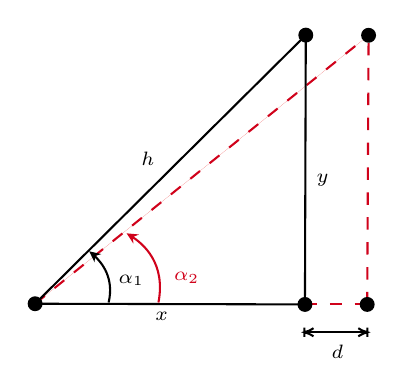
\begin{tikzpicture}[x=0.75pt,y=0.75pt,yscale=-1,xscale=1]
%uncomment if require: \path (0,300); %set diagram left start at 0, and has height of 300

%Straight Lines [id:da607447387383602] 
\draw [color={rgb, 255:red, 208; green, 2; blue, 27 }  ,draw opacity=1 ][fill={rgb, 255:red, 230; green, 39; blue, 39 }  ,fill opacity=1 ] [dash pattern={on 4.5pt off 4.5pt}]  (195.25,185.75) -- (355.92,56.42) ;
%Straight Lines [id:da27148655997396476] 
\draw [color={rgb, 255:red, 208; green, 2; blue, 27 }  ,draw opacity=1 ] [dash pattern={on 4.5pt off 4.5pt}]  (355.25,186.08) -- (355.92,56.42) ;
%Straight Lines [id:da7571554100323626] 
\draw [color={rgb, 255:red, 208; green, 2; blue, 27 }  ,draw opacity=1 ] [dash pattern={on 4.5pt off 4.5pt}]  (325.25,186.08) -- (355.25,186.08) ;
%Shape: Circle [id:dp7176360013947902] 
\draw  [fill={rgb, 255:red, 0; green, 0; blue, 0 }  ,fill opacity=1 ] (192.17,185.75) .. controls (192.17,184.05) and (193.55,182.67) .. (195.25,182.67) .. controls (196.95,182.67) and (198.33,184.05) .. (198.33,185.75) .. controls (198.33,187.45) and (196.95,188.83) .. (195.25,188.83) .. controls (193.55,188.83) and (192.17,187.45) .. (192.17,185.75) -- cycle ;
%Shape: Circle [id:dp24601699255953835] 
\draw  [fill={rgb, 255:red, 0; green, 0; blue, 0 }  ,fill opacity=1 ] (322.17,186.08) .. controls (322.17,184.38) and (323.55,183) .. (325.25,183) .. controls (326.95,183) and (328.33,184.38) .. (328.33,186.08) .. controls (328.33,187.79) and (326.95,189.17) .. (325.25,189.17) .. controls (323.55,189.17) and (322.17,187.79) .. (322.17,186.08) -- cycle ;
%Shape: Circle [id:dp906352155237646] 
\draw  [fill={rgb, 255:red, 0; green, 0; blue, 0 }  ,fill opacity=1 ] (322.58,56.33) .. controls (322.58,54.63) and (323.96,53.25) .. (325.67,53.25) .. controls (327.37,53.25) and (328.75,54.63) .. (328.75,56.33) .. controls (328.75,58.04) and (327.37,59.42) .. (325.67,59.42) .. controls (323.96,59.42) and (322.58,58.04) .. (322.58,56.33) -- cycle ;
%Straight Lines [id:da11648942189495237] 
\draw    (195.25,185.75) -- (325.67,56.33) ;
%Straight Lines [id:da26461786666325793] 
\draw    (195.25,185.75) -- (325.25,186.08) ;
%Straight Lines [id:da23855514855400362] 
\draw    (325.25,186.08) -- (325.67,56.33) ;
%Curve Lines [id:da7632155654947097] 
\draw    (230.67,185.17) .. controls (233.4,173.41) and (227.62,166.14) .. (223.61,162.44) ;
\draw [shift={(221.33,160.5)}, rotate = 38.66] [fill={rgb, 255:red, 0; green, 0; blue, 0 }  ][line width=0.08]  [draw opacity=0] (5.36,-2.57) -- (0,0) -- (5.36,2.57) -- (3.56,0) -- cycle    ;
%Shape: Circle [id:dp2379888459592604] 
\draw  [fill={rgb, 255:red, 0; green, 0; blue, 0 }  ,fill opacity=1 ] (352.17,186.08) .. controls (352.17,184.38) and (353.55,183) .. (355.25,183) .. controls (356.95,183) and (358.33,184.38) .. (358.33,186.08) .. controls (358.33,187.79) and (356.95,189.17) .. (355.25,189.17) .. controls (353.55,189.17) and (352.17,187.79) .. (352.17,186.08) -- cycle ;
%Shape: Circle [id:dp4318264592938509] 
\draw  [fill={rgb, 255:red, 0; green, 0; blue, 0 }  ,fill opacity=1 ] (352.83,56.42) .. controls (352.83,54.71) and (354.21,53.33) .. (355.92,53.33) .. controls (357.62,53.33) and (359,54.71) .. (359,56.42) .. controls (359,58.12) and (357.62,59.5) .. (355.92,59.5) .. controls (354.21,59.5) and (352.83,58.12) .. (352.83,56.42) -- cycle ;
%Curve Lines [id:da5116933081563226] 
\draw [color={rgb, 255:red, 208; green, 2; blue, 27 }  ,draw opacity=1 ]   (254.67,185.17) .. controls (258.31,166.13) and (247.36,156.97) .. (241.79,153.34) ;
\draw [shift={(239.33,151.83)}, rotate = 30.96] [fill={rgb, 255:red, 208; green, 2; blue, 27 }  ,fill opacity=1 ][line width=0.08]  [draw opacity=0] (5.36,-2.57) -- (0,0) -- (5.36,2.57) -- (3.56,0) -- cycle    ;
%Straight Lines [id:da10028566006612083] 
\draw    (325,199.5) -- (355.33,199.5) ;
\draw [shift={(355.33,199.5)}, rotate = 180] [color={rgb, 255:red, 0; green, 0; blue, 0 }  ][line width=0.75]    (0,2.24) -- (0,-2.24)(4.37,-1.96) .. controls (2.78,-0.92) and (1.32,-0.27) .. (0,0) .. controls (1.32,0.27) and (2.78,0.92) .. (4.37,1.96)   ;
\draw [shift={(325,199.5)}, rotate = 0] [color={rgb, 255:red, 0; green, 0; blue, 0 }  ][line width=0.75]    (0,2.24) -- (0,-2.24)(4.37,-1.96) .. controls (2.78,-0.92) and (1.32,-0.27) .. (0,0) .. controls (1.32,0.27) and (2.78,0.92) .. (4.37,1.96)   ;

% Text Node
\draw (234,170.33) node [anchor=north west][inner sep=0.75pt]  [font=\scriptsize] [align=left] {$\displaystyle \alpha _{1}$};
% Text Node
\draw (260.67,169) node [anchor=north west][inner sep=0.75pt]  [font=\scriptsize] [align=left] {$\displaystyle \textcolor[rgb]{0.82,0.01,0.11}{\alpha }\textcolor[rgb]{0.82,0.01,0.11}{_{2}}$};
% Text Node
\draw (336.67,204) node [anchor=north west][inner sep=0.75pt]  [font=\scriptsize] [align=left] {$\displaystyle d$};
% Text Node
\draw (251.67,188.33) node [anchor=north west][inner sep=0.75pt]  [font=\scriptsize] [align=left] {$\displaystyle x$};
% Text Node
\draw (329.33,122) node [anchor=north west][inner sep=0.75pt]  [font=\scriptsize] [align=left] {$\displaystyle y$};
% Text Node
\draw (245,111) node [anchor=north west][inner sep=0.75pt]  [font=\scriptsize] [align=left] {$\displaystyle h$};


\end{tikzpicture}
